% Ergebnisse und Analyse.tex

% Ergebnisse und Analyse Diagramme.tex

\newcommand{\MergesortMesswerte}{%
    \addplot[blue, mark=*] coordinates {
            (25000000,3017372600)
            (50000000,6315632400)
            (100000000,12777405700)
            (200000000,27203738300)
            (400000000,56441153000)
        };
    \addlegendentry{Mergesort}
}

\newcommand{\QuicksortMesswerte}{%
    \addplot[green, mark=*] coordinates {
            (25000000,1528071600)
            (50000000,3248990900)
            (100000000,6653966800)
            (200000000,13778762100)
            (400000000,29074726600)
        };
    \addlegendentry{Quicksort}
}

\newcommand{\GrundlegendeLaufzeitenAbhaengigVonDerArraygroesseDiagrammA}{%
    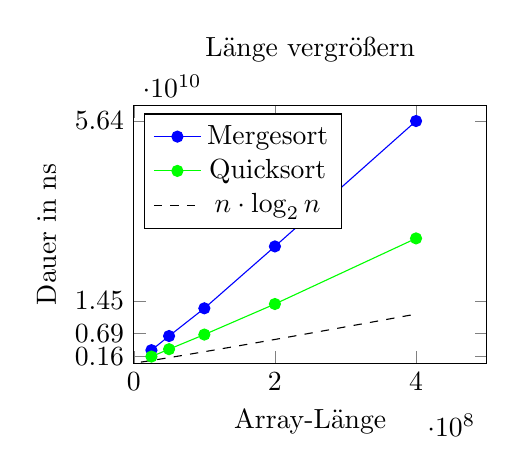
\begin{tikzpicture}
        \begin{axis}[
                title style={yshift=1.5ex},
                width=0.5\textwidth,
                height=0.4\textwidth,
                xlabel={Array-Länge},
                ylabel={Dauer in ns},
                title={Länge vergrößern},
                xmin=0, xmax=5 * 10^8,
                ymin=0*10^6, ymax=6*10^10,
                grid style=dashed,
                legend pos=north west,
                ytick={1609541400,6854920900,14495472700,56441153000},
                % xtick={2^21,2^23,2^24,2^25},
                % xticklabels={$2^{21}$, $2^{23}$, $2^{24}$, $2^{25}$},
                % scaled x ticks=false,
                % scaled y ticks=false,
            ]
            \MergesortMesswerte
            \QuicksortMesswerte
            % n*log2(n)
            \addplot[black, dashed,domain=1e7:4e8, samples=100] {x*log2(x)};
            \addlegendentry{$n \cdot \log_2 n$}
            % % n
            % \addplot[red, dashed,domain=1e7:4e8, samples=100] {x};
            % \addlegendentry{$n$}
            % % log2(n)
            % \addplot[green, domain=1e7:4e8, samples=100] {log2(x)};
            % \addlegendentry{$\log_2 n$}
        \end{axis}
    \end{tikzpicture}%
}

\newcommand{\GrundlegendeLaufzeitenAbhaengigVonDerArraygroesseDiagrammB}{%
    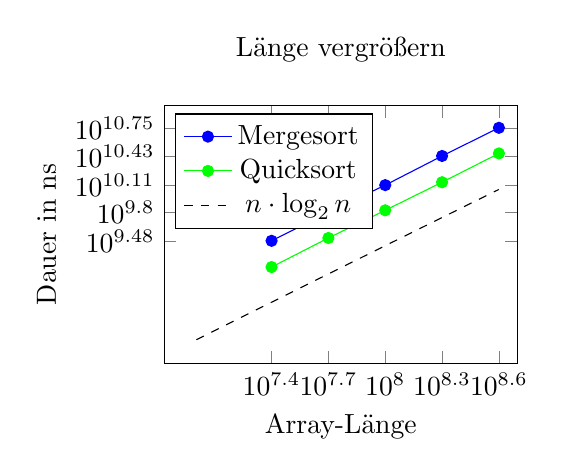
\begin{tikzpicture}
        \begin{axis}[
                title style={yshift=1.5ex},
                width=0.5\textwidth,
                height=0.4\textwidth,
                xlabel={Array-Länge},
                ylabel={Dauer in ns},
                title={Länge vergrößern},
                xmin=0, xmax=5 * 10^8,
                ymin=0*10^6, ymax=1*10^11,
                grid style=dashed,
                legend pos=north west,
                xmode=log,
                log basis x=10,
                xtick=data,
                ymode=log,
                log basis y=10,
                ytick=data,
                % xtick={2^21,2^23,2^24,2^25},
                % xticklabels={$2^{21}$, $2^{23}$, $2^{24}$, $2^{25}$},
                % scaled x ticks=false,
                % scaled y ticks=false,
            ]
            \MergesortMesswerte
            \QuicksortMesswerte
            % n*log2(n)
            \addplot[black, dashed,domain=1e7:4e8, samples=100] {x*log2(x)};
            \addlegendentry{$n \cdot \log_2 n$}
        \end{axis}
    \end{tikzpicture}%
}


% Definiere Variablen
% \newcommand{\Messziel}{Messziel}

% % ----------------------
% % 4. Ergebnisse und Analyse
% % ----------------------
% \newpage
% \chapter{Ergebnisse und Analyse}
% \section{Grundlegende Laufzeiten abhängig von der Arraygröße}
% \subsection{Messziel} % Einleitung
% \subsection{Erwartung}
% \subsection{Diagramm}
% \subsection{Analyse und Interpretation}
% \newpage
% \section{Einfluss des Listentyps} % Listentyps: Zufall, Sortiert, InvertiertSortiert, FastSortiert, Dupliziert
% \subsection{Messziel} % Einleitung
% \subsection{Erwartung}
% \subsection{Diagramm}
% \subsection{Analyse und Interpretation}
% \newpage
% \section{Einfluss der Arraygröße im Detail}
% \subsection{Messziel} % Einleitung
% \subsection{Erwartung}
% \subsection{Diagramm}
% \subsection{Analyse und Interpretation}
% \newpage
% \section{Tiefenbasierte Thread-Erzeugung}
% \subsection{Messziel} % Einleitung
% \subsection{Erwartung}
% \subsection{Diagramm}
% \subsection{Analyse und Interpretation}
% \newpage
% \section{Workerthreads}
% \subsection{Messziel} % Einleitung
% \subsection{Erwartung}
% \subsection{Diagramm}
% \subsection{Analyse und Interpretation}
% \newpage
% \section{Vergleich der Threading-Methoden}
% \subsection{Messziel} % Einleitung
% \subsection{Erwartung}
% \subsection{Diagramm}
% \subsection{Analyse und Interpretation}
% \newpage
% \section{Einfluss des Datentyps der Liste} % Listenart: int, string
% \subsection{Messziel} % Einleitung
% \subsection{Erwartung}
% \subsection{Diagramm}
% \subsection{Analyse und Interpretation}
% % \section{Debug Vs Release}

% % ----------------------
% % 4. Ergebnisse und Analyse
% % ----------------------
% \chapter{Ergebnisse und Analyse}
% \section{Grundlegende Laufzeiten abhängig von der Arraygröße}

% \subsection{Messziel} % Einleitung
\newcommand{\GrundlegendeLaufzeitenAbhaengigVonDerArraygroesseMessziel}{
    Das Messziel besteht darin, die Abhängigkeit des seriellen Algorithmus von der Arraygröße grafisch darzustellen.
    Dadurch können diese Ergebnisse später mit den nicht-seriellen Varianten verglichen werden.
    Gleichzeitig dient dies als einfacher Einstieg in das Thema.
}

% \subsection{Erwartung}
\newcommand{\GrundlegendeLaufzeitenAbhaengigVonDerArraygroesseErwartung}{
    Da die durchschnittliche Laufzeit \(O(n \log n)\) beträgt, erwarte ich eine logarithmische Laufzeiterhöhung bei wachsender Arraygröße.
}
% \subsection{Diagramm}
\newcommand{\GrundlegendeLaufzeitenAbhaengigVonDerArraygroesseDiagramm}{
    \GrundlegendeLaufzeitenAbhaengigVonDerArraygroesseDiagrammA
    \GrundlegendeLaufzeitenAbhaengigVonDerArraygroesseDiagrammB
    \newline
    \GrundlegendeLaufzeitenAbhaengigVonDerArraygroesseDiagrammC
}

% \subsection{Analyse und Interpretation}
\newcommand{\GrundlegendeLaufzeitenAbhaengigVonDerArraygroesseAnalyse}{
    In den ersten zwei Diagrammen ist die Veränderung der Laufzeit zu sehen, wenn die Listengröße fünfmal verdoppelt wird und bei \(2.5 \cdot 10^7\) startet.
    Beim zweiten Diagramm sind die Achsen logarithmisch dargestellt, da dies die Darstellung und den Vergleich der Laufzeiten erleichtert.
    \newline
    Unter diesen beiden Diagrammen befindet sich ein drittes Diagramm, in dem die gemessenen Laufzeiten ebenfalls logarithmisch dargestellt sind und der Größenbereich von \(1\) bis \(800\,000\) betrachtet wird.
    \newline
    Anhand dieser Diagramme ist deutlich erkennbar, dass sowohl Mergesort als auch Quicksort tatsächlich eine Laufzeit von
    \(O(n \log n)\) besitzen.
    \newline
    Zudem ist erkennbar, dass Mergesort etwa doppelt so lange benötigt wie Quicksort und dass Quicksort näherungsweise eine Laufzeit von
    \(2 \cdot n \log_2(n)\) aufweist.
    Aus diesen Beobachtungen lässt sich ableiten, dass der Partitionierungsschritt eine Laufzeit von etwa \(2n\) besitzt, während der Merge-Schritt näherungsweise eine Laufzeit von \(4n\) aufweist.
    Zur Vereinfachung der Betrachtung wird jedoch bei beiden Algorithmen weiterhin von \(n\) ausgegangen.
    \newline
    Da eine lineare Laufzeit auf einen Blick leichter zu interpretieren ist, wurde zusätzlich die Funktion \(32n\) eingezeichnet.
    Anhand dieser Funktion ist erkennbar, dass sie im untersuchten Zahlenbereich von \(1\) bis \(4 \cdot 10^8\) teilweise sogar eine genauere Abschätzung liefert als \(n \log_2(n)\).
    Daraus folgt, dass von einer begründeten Mindestlaufzeit von \(32n\) ausgegangen werden kann.
    \newline
    Abschließend ist anzumerken, dass alle Messungen mit einer Laufzeit von kleiner oder gleich \(10^4\,\text{ns}\) aufgrund der Messtoleranz nur eine eingeschränkte Aussagekraft besitzen.
    Zwar kann mit \texttt{chrono} auf eine Auflösung von \(100\,\text{ns}\) genau gemessen werden, dennoch verbleiben natürliche Schwankungen, die insbesondere im Bereich von \(10^4\,\text{ns}\) einen erheblichen Einfluss auf die Messergebnisse haben.
}